% this file is called up by thesis.tex
% content in this file will be fed into the main document

\chapter{Outage Modelling} % top level followed by section, subsection
\label{ch:OM}

\begin{textsl}
{\small Hosting software applications in a Cloud based infrastructure represents challenges for micro teams and (SMEs), due to the variety of ways in which production outages can occur. We consider both the inter-arrival and service (repair) times for outage events in a framework where these downtimes are used to re-focus DevOps resources. Using an enterprise dataset, we address the question of how inter-arrival and service times of outage events are distributed and what relationship the service times have with different types of failures that can occur in a Cloud data centre. The proposed framework can aid micro teams and SMEs to maintain a highly available On-Demand service infrastructure, with limited resources.}
\end{textsl}

\vspace*{1cm}

%\adjustmtc

%\minitoc
% ----------------------- contents from here ------------------------


% % % % % % % % % % % % % % % % % % % % % % % % % % % % % % % % % % % % % % % % % % % % % % % % % % % % % %
%---------------------------------------- INTRODUCTION ----------------------------------------------------
% % % % % % % % % % % % % % % % % % % % % % % % % % % % % % % % % % % % % % % % % % % % % % % % % % % % % %
\section{Introduction}
For the micro team and SME the adoption of Cloud technology no easy task. Due to resource constraints and myriad of failure patterns, small teams face challenges in providing a reliable and stable service platform for their customer's needs \cite{carcary2014adoption}. 

One way to provide services with an elevated market reach is through a Software as a Service (SaaS) model. This Cloud-based approach is seen as a shift away from highly complex bespoke solutions, to more focused and cost effective solution \cite{Cloudbook2015}. As customers demand highly effective services to solve their business problems, a Cloud platform can help keep pace with these needs. A single delivery platform is used to host multiple software solutions and services. \par

However SMEs face a number of key challenges when embracing a Cloud service model, especially in the area of reliability and maintainability. Recent work has highlighted a number of challenges, which include: outage frequency and duration. Almost all SMEs (93\%) employ less than 10 people \cite{europa2015sme}, therefore in this chapter we analyse the factors that may impede reliability especially for businesses with low levels of resources. \par

In this chapter we describe a framework, that the SME can use to best manage their limited pool of resources. The core idea of this framework is for Cloud operations teams to focus on areas with high outage times (typically areas with high manual processes) to reduce the overall outage time. This chapter contains two studies of software outage data from a large enterprise dataset. Through study of this outage event data we show a) how to first model the inter-arrival time of Cloud outage events. b) by modelling the service times of outages which types of outage events take the longest to resolve. We also consider why having standardised homogeneous data centres are key to reducing outage times, and how application types play a role in the duration of outage remediation. \par

For businesses who provide their Cloud platform to allow companies to host services or solutions, this is known as Platform as a Service (PaaS). These providers allow for multi-tenancy. It is proposed that  high-level outage data could be shared between organisations to triangulate cross application outage events. \par

\section{Case study 3 - Outage inter-arrival time modelling}
The study presented in this case study examines approximately 250 Cloud outage events from a large enterprise system. The data was collected over a 12-month period (Jan -- Dec) and is comprised of four main components: E-mail, Collaboration, Social and Business Support System (BSS). Additionally the class of outage have been grouped into the following main categories: Configuration/Manual Process, Contention/Concurrency, Disaster Recovery, Network and Hardware/Other. The systems have been deployed within three data centres and are used by customers globally. The software is developed in Java and runs on Linux. \par 

Product development follows a Continuous delivery (CD) development model whereby small component features are released to the public on a monthly basis. For each outage event we have access to the full outage report, but we particularly focus on the time duration between outage events (inter-arrival time). We also consider the inter-arrival time when grouped against component, outage type and data centre. 

Our third case study aims to answer the following question: What distribution is best suited to model the inter-arrival time of Cloud outage events recorded in our dataset. Second, does the inter-arrival time distribution vary by component? Third, does the inter-arrival time distribution differ by failure category? Fourth, does the inter-arrival time distribution differ by data centre? In order to answer these four questions, this study is broken down into the following attributes: outage distribution, outage component, outage failure category and  data centre location.

\subsection{Outage service time distribution}

Probability distributions are used in statistics to assign a likelihood of an event taking place. In the case of Cloud outage events, by analysing the distribution of all outage, it may be possible to fit a known distribution to our dataset. If a distribution can be fitted, these distribution properties can be used to infer the most likely outcome of an outage event. For example a probability distribution could be used to infer the likelihood duration between outage events. An outage distribution is plotted for the complete set of outages. To determine whether our dataset can be modelled by a known distribution type, a parametric approach is considered (i.e. MLE \cite{pearson1894contributions}). Using the R package 
fitdistrplus \cite{fitdistrplus} we fitted many known distributions (e.g. exponential, gamma, log-normal and Weibull)
 against our dataset. For distribution validation we used the R library ADGofTest \cite{ADGoF} against a number of likely distributions types. 

\subsection{Outage component}

Recognising component failures gives an understanding of a) what components are more likely to contribute to an outage event and b) the relative duration between each event with respect to a component. For example, operations teams may have various probes to determine if an event is likely to cause a failure. Development and test teams may have a suite of test cases to find a certain class of issue. Outage events can provide operations teams with an understanding of potential gaps in their probes and monitoring solutions. Furthermore, for development and test teams outage events can highlight gaps in test coverage, irrespective of whether this gap is at unit, functional, or performance/system level. There are four main components: BSS, collaboration, email and social. For this case study we categorised our software components as follows: BSS/social, collaboration, email and mixed (where multiple components where involved). \par

\subsection{Outage type}
Grouping Cloud outages by type is useful exercise. Using these sub categories: Configuration/Manual, Contention/Concurrency, Disaster Recovery, Network and Hardware/Other, we can infer whether the duration time between each type outage is similar.

Configuration/Manual errors involve situations where a configuration change is made from one value to another that causes a software or hardware component to behave abnormally. For example a Load Balancer setting could be changed manually which reduces the throughput from Gigabits to Megabits which could greatly reduce the infrastructures's ability to manage incoming traffic.\par

Contention/Concurrency outages refer to a class of issue, that is triggered through normal operations on the underlying server component code. These issues are triggered due to the inability of the code to handle either concurrent or parallel usage. Software defects may include issues related to contention under load (e.g. memory leaks, high Disk I/O, CPU usage), concurrency (e.g. deadlocks) or miscellaneous race conditions. \par

Disaster Recovery errors typically involve scenarios where system load was required to move from one application server or database to another. In some situations the session data may not transfer correctly and cause a failure of routine operations. \par

A network error relates to a class of failure outside of misconfiguration or a hardware failure within the network infrastructure. Network failures can typically present themselves as intermittent temporary network outages, high latency/packet loss conditions or congestion based on overloading of available bandwidth. As Cloud data centres contain a number of distributed systems, having a reliable network infrastructure is highly desirable. \par

A Hardware/Other failure relates to a class of problem, which causes a piece of hardware to fail. These failures relate to a malfunction within the electronic circuits or electromechanical components (disks, tapes) of a computer system. Recovery from a hardware failure requires repair or replacement of the offending part. Additionally the error may relate to some miscellaneous type of error that is not part of the four main failure categories. \par

\subsection{Outage by data centre location}

Understanding the measure of outage events at a data centre level can highlight whether a specific data centre is a factor in the duration and distribution of outage events raised. There are three data centres in our dataset: data centre A (High usage), data centre B (Low usage) and data centre C (Medium usage). Understanding whether the duration between outage events are similar or different in each data centre can be a useful data point for DevOps teams.

\subsection{Limitations of dataset}

The outage events that form part of this study are from an enterprise Cloud system. The inter-arrival times of these outage events are applicable to the software domain of BSS, collaboration, email and social software. While we hope these examples will be representative of social and collaboration based software, it seem unlikely they will be
typical of all types of Cloud based software.

\subsection{Results - outage inter-arrival time distribution}

\begin{table}[!ht]\centering
\caption{Summary of Anderson-Darling GoF statistics.}
\label{tab:chap4tab1}
\begin{tabular}{| C{4cm} | C{4cm} | C{4cm} |} \hline 
\textbf{Distribution name}  & \textbf{AD statistic} & \textbf{p-value}
\\ \hline Pareto & 0.661  & 0.592
\\ \hline Weibull & 0.975 & 0.371
\\ \hline log-logistic & 1.823  & 0.115
\\ \hline log-normal & 3.039  & 0.026 
\\ \hline exponential & 3.110  & 0.024
\\ \hline gamma & 6.034  & 9.347e-04 
\\ \hline logistic & 12.819 & 2.765e-06
\\ \hline
\end{tabular}
\end{table}

\begin{figure}[ht!]\centering
\caption{Four goodness-of-fit plots for Weibull, log-logistic and Pareto distributions fitted to the inter-arrival times from the Cloud outage data set}
\label{fig:chap4fig1}
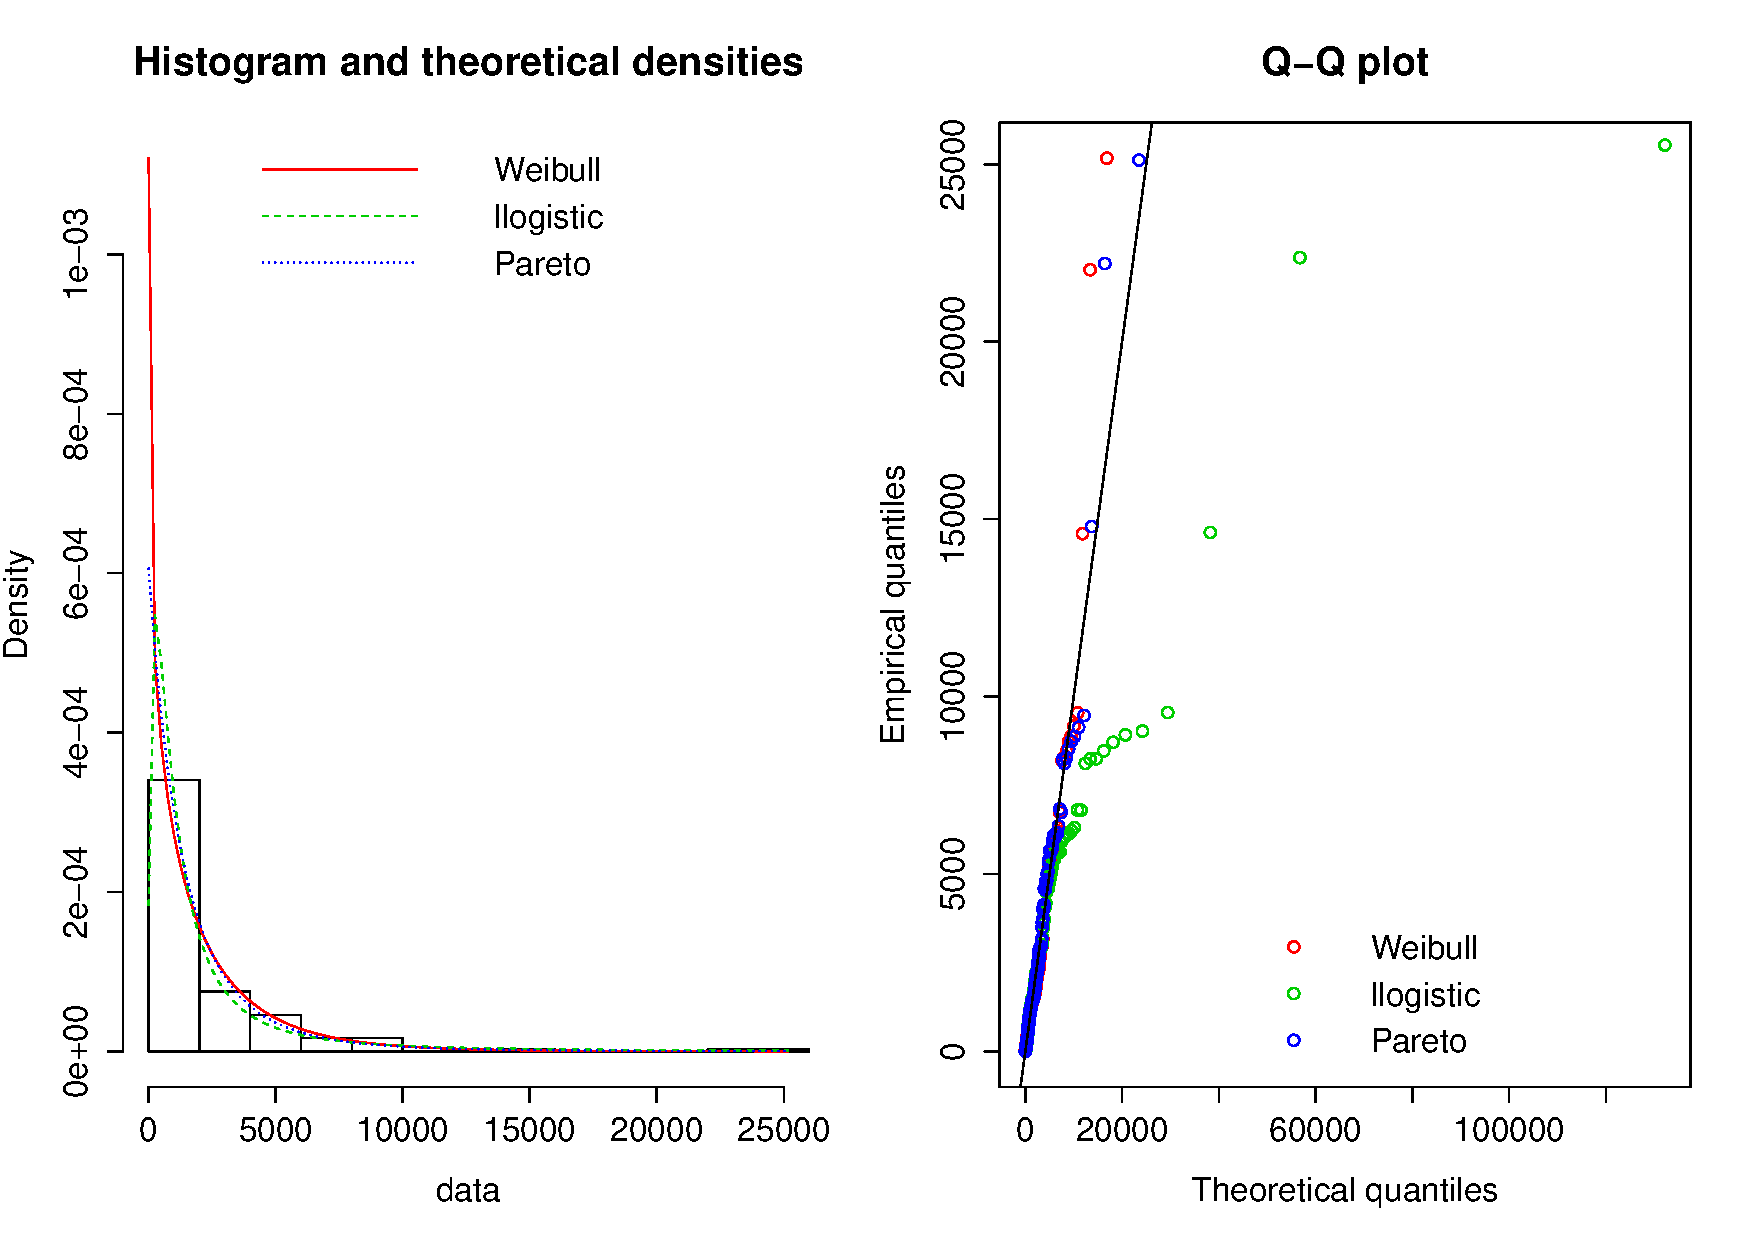
\includegraphics[width=14cm, height=7cm]{graphs/inter-arrival/Graphs1.pdf}
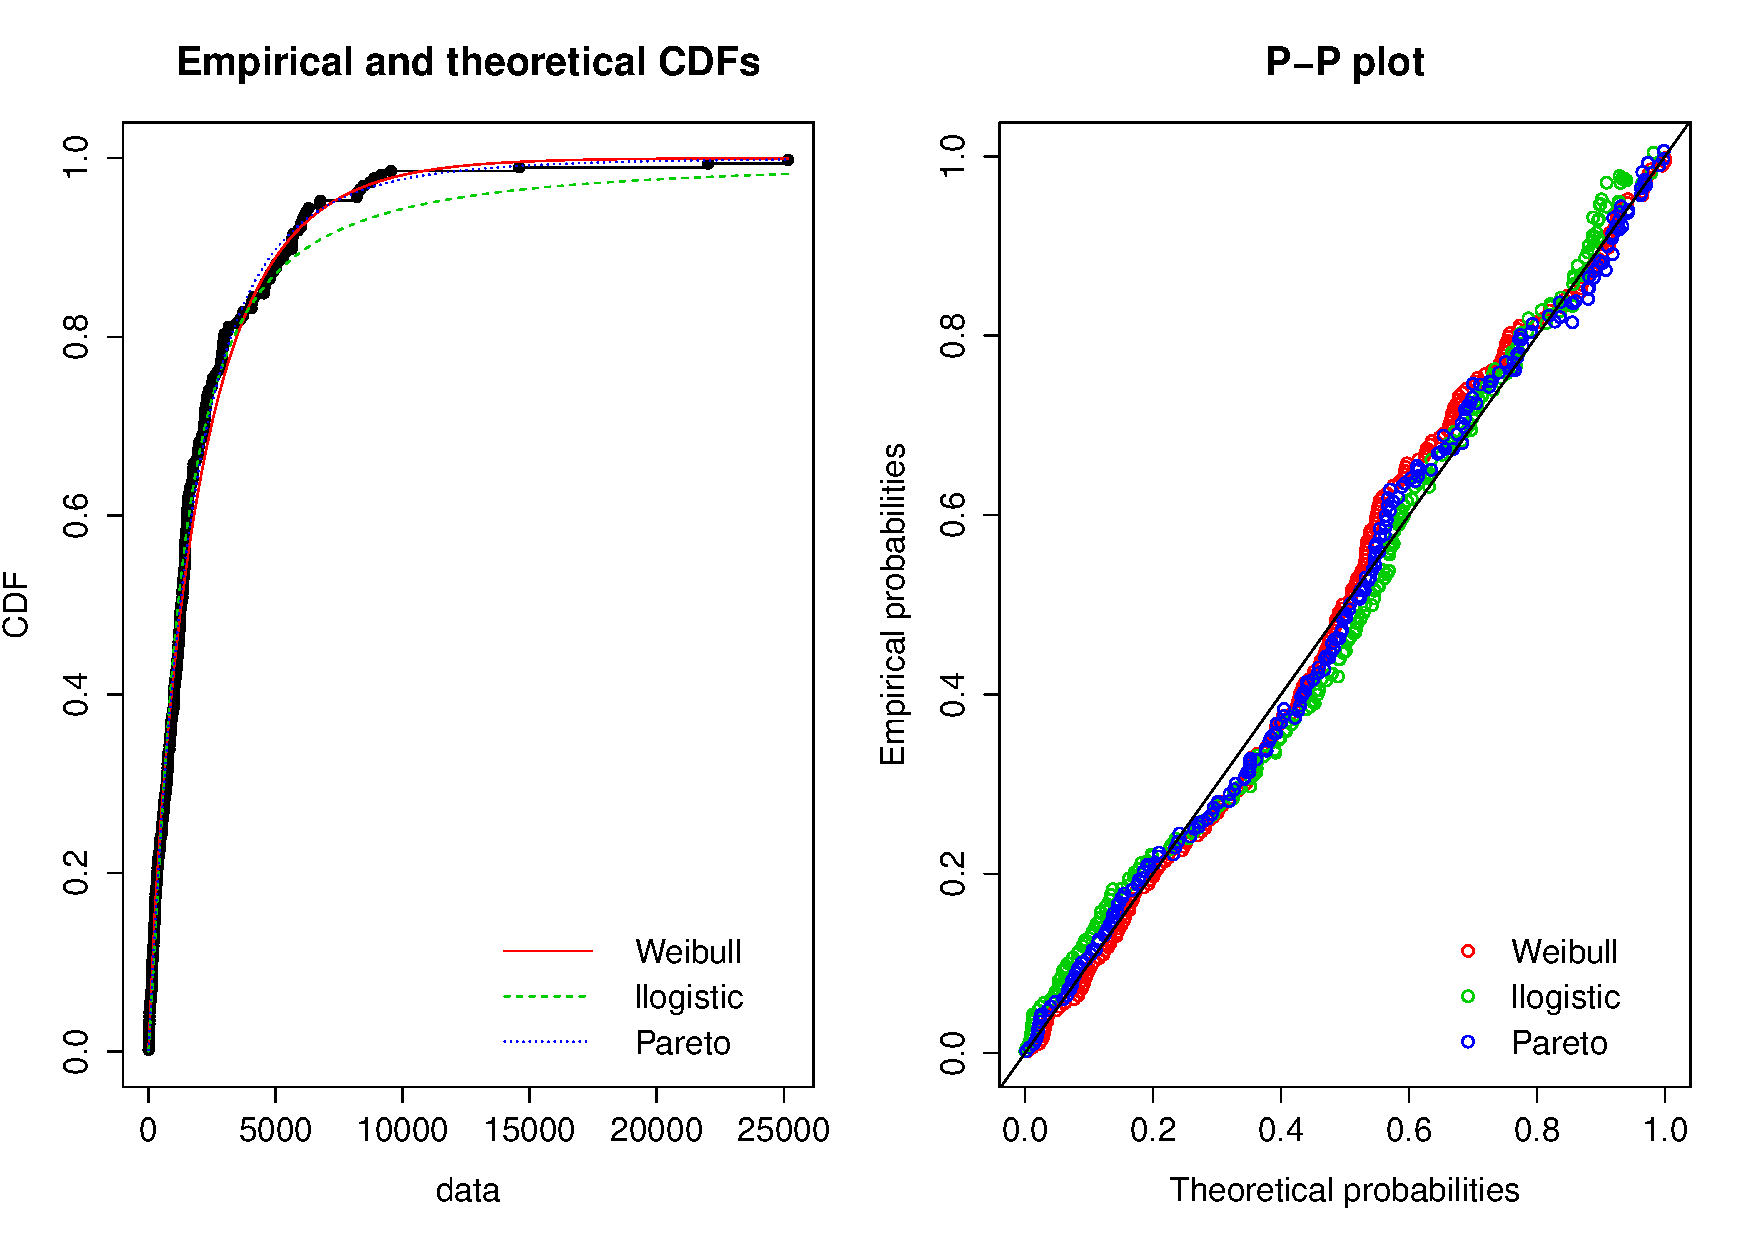
\includegraphics[width=14cm, height=7cm]{graphs/inter-arrival/Graphs2.pdf}
\end{figure}

Table \ref{tab:chap4tab1} shows the summary results for our distribution fitting exercise. Seven distributions types were fitted against our data set. The table is sorted from highest to lowest p-value. Pareto, Weibull and log-logistic all have p-values above 0.05, which is a cutoff to for our hypothesis test. Figure \ref{fig:chap4fig1} shows four goodness-of-fit plots (PDF, CDF,  quantile-quanltile plot and probability plot) for the top three performing distributions.


\subsection{Results - outage component}

\begin {table}
\begin{center}
\caption {Summary statistics for outage inter-arrival times by component with Pareto GoF} 
\label{tab:chap4tab2}
\begin{tabular}{| C{2.5cm} | C{2.4cm} | C{2.9cm} | C{2cm} | C{2cm} |} \hline 
\textbf{Statistic} & \textbf{BSS/Social} & \textbf{Collaboration} & \textbf{Email} & \textbf{Mixed}
\\ \hline Samples & 16 & 34 & 150 & 43
\\ \hline \% Samples & 7 & 14 & 62 & 18
\\ \hline  Mean & 2362.41 & 2334.26 & 1988.90 & 2567.73
\\ \hline  Std Dev & 2327.04 & 3106.15 & 2607.27 & 4096.10
\\ \hline  Median & 1338 & 1124 & 1262.50 & 1420
\\ \hline  Skew & 1.12 & 2.36 & 3.93 & 4.43
\\ \hline AD GoF (p) & 0.32 & 0.84 & 4.0e-06 & 0.83
\\ \hline 
\end{tabular}
\end{center}
\end{table}

Table \ref{tab:chap4tab2} provides a summary of outage inter-arrival times grouped by component. E-Mail recorded the highest proportion of all outages with the BSS/social category recording the lowest proportion of outages.

Also included in the table are the AD GoF p-values for each sub-group of outage failures. It is noted that all sub-groups have a p-value above 0.05, with the exception of email. 

\subsection{Results - outage type}

\begin {table}
\begin{center}
\caption {Summary statistics for outage inter-arrival times by outage type with Pareto GoF} 
\label{tab:chap4tab3}
\begin{tabular}{| C{2.02cm} | C{1.9cm} | C{1.9cm} | C{1.9cm} | C{1.78cm} | C{1.9cm} |} \hline 
\textbf{Statistic} & \textbf{Configuration} & \textbf{Contention} & \textbf{Disaster} & \textbf{Network} & \textbf{Hardware}
\\ & \textbf{Manual} & \textbf{Concurrency} & \textbf{Recovery} & & \textbf{Other}
\\ \hline \# Samples & 74 & 64 & 35 & 48 & 21
\\ \hline  \% Samples & 30 & 26 & 14 & 20 & 9
\\ \hline Mean & 1782.57 & 2342.88 & 2719.71 & 1945.13 & 2510.86
\\ \hline Std Dev & 2488	& 2336.87 & 4316.33 & 2325.02 & 2346.90
\\ \hline Median & 1019 & 1429 & 1438 & 1087.50 & 1704
\\ \hline  Skew & 5.85 & 1.41 & 3.41 & 1.89 & 0.91
\\ \hline AD GoF (p) & 0.42 & 0.81 & 0.75 & 1.25e-05 & 0.54
\\ \hline 
\end{tabular}
\end{center}
\end{table}

Table \ref{tab:chap4tab3} provides a summary of outage inter-arrival times pooled by outage type. Configuration/Manual recorded the highest proportion of all outages while the Hardware/Other category recording the lowest proportion of outages.

Also provided are the AD GoF p-values for each sub-group of outage failures. It is noted that all sub-groups have a p-value above 0.05, with the exception of network. 

\subsection{Results - data centre location}

\begin {table}
\begin{center}
\caption {Summary statistics for outage inter-arrival times by data centre with Pareto GoF} 
\label{tab:chap4tab4}
\begin{tabular}{| C{3cm} | C{3cm} | C{3cm} | C{3cm} |} \hline 
\textbf{Statistic} & \textbf{Data centre A} & \textbf{Data centre B}  & \textbf{Data centre C} 
\\ \hline Samples & 159 & 24 & 51 
\\ \hline \% Samples & 65 & 10 & 21
\\ \hline Mean & 2439.74	& 2280.21 	& 1348.12
\\ \hline Std Dev & 3315.80	& 2920.74 & 1500.80
\\ \hline Median & 1395	& 1480.5	& 909
\\ \hline Skew & 3.76	& 3.48	& 1.84 
\\ \hline AD GoF (p) & 0.54 & 0.79 & 1.18e-05 
\\ \hline 
\end{tabular}
\end{center}
\end{table}

Table \ref{tab:chap4tab4} show a summary of outage inter-arrival times pooled by data centre. Data centre A recorded the highest proportion of all outages while the data centre B category recording the lowest proportion of outages. The proportion of outages follows our intuition that data centres with the highest usage have the highest proportion of failures.

Also shown are the AD GoF p-values for each sub-group of outage failures. It is noted that all sub-groups have a p-value above 0.05, with the exception of data centre C. 


\subsection{Discussion - outage inter-arrival time distribution}

Table  \ref{tab:chap4tab1} shows that Pareto has the highest p-value for the Anderson-Darling test, followed by log-logistic and Weibull. If we consider the hypothesis, do the inter-arrival times belong to a specific distribution family? In four cases we reject the hypothesis for log-normal, gamma, exponential and logistic, due to the p-value being less than 0.05. Using the p-value alone it is clear that the Pareto distribution is the best fitting distribution. Using graphical means as a second frame of reference, figure \ref{fig:chap4fig1} shows the goodness of fit plots for the three best fitted distributions. 

In the histogram plot with fitted curve we can see that the Pareto curve fits the curve at lower values better than the other two distributions. Additionally the The quantile-quanltile plot shows that the Pareto distribution more closely models the data set even for extreme values. With a better fit at both the head and the tail of the data, the Pareto distribution is clearly the best choice to model the inter-arrival times of our Cloud outage data.

\subsection{Discussion - outage component}

Table \ref{tab:chap4tab2} provides summary details of outages by component. It was observed that mixed components had the highest mean inter-arrival time with 2567.73 minutes, followed by BSS/social, Collaboration with 2362.41 \& 2334.26 respectively and Email with 1988.90 minutes. Intuitively mixed components also had the highest median, skew and standard deviation. In three of the component sub-classes (BSS/Social, Collaboration and mixed) the fit to a Pareto distribution was above the 0.05 p-value criterion. This indicates that it is reasonable to assume the inter-arrival times from these three sub-categories can be modelled by a Pareto distribution. However for the Email sub-class the p-value computed was well below the 0.05. We conclude that the Pareto distribution is not a reasonable choice to model outage inter-arrival times for Email alone.

Based on these results it is clear that the email component has the highest proportion of outages. Moreover, the email component has the lowest mean inter-arrival time. DevOps teams should review the root causes for each email failure to determine each and every failure trigger. This will provide more information to understand why email outages happen more frequently and with shorter duration between failures than any other component. 

Secondly the results show that mixed components have the highest mean outage time. Given the complex nature of multi-component outages, it is logical to suggest that while these types of were the second most frequent, these types of outage take longer to propagate. This is due in part to the number of systems across the Cloud infrastructure that would need to fail. DevOps teams can triangulate these types of mixed outage failure across type and data centre to determine persistent failure patterns.

Finally, while the Pareto distribution is shown to be a reasonable distribution to model outage inter-arrival times of our entire dataset, we note that when working with sub-categories, this intuition is not exclusively true.

\subsection{Discussion - outage type}

Examining outages by type gives a deeper understanding of how the inter-arrival times of outages vary by type. Table \ref{tab:chap4tab3} provides summary results. \par

Of immediate interest is the Configuration/Manual outage type. This category scored the highest number of outages, the shortest inter-arrival mean time and the lowest inter-arrival median duration. It is clear that outages related to Configuration/Manual occurred most frequently during the twelve month analysis window. It is worth noting that the Configuration/Manual skew was the highest indicating considerable variability between consecutive outage events. Finally we observed that the Configuration/Manual inter-arrival times alone were a good fit for a Pareto distribution with a p-value of 0.42.

Contention/Concurrency and Network types recorded the 2nd and 3rd highest number of outages. The mean inter-arrival time for Contention/Concurrency was approximately 400 seconds long than that of Network. This indicates that while Contention/Concurrency outage events happen with a greater degree of regularity than Network issues, on average the duration between subsequent events is much greater. Finally we note that Contention/Concurrency had a highest computed p-value fit to a Pareto distribution with 0.81. However it was also noted that the p-value for Network was below the 0.05 significance level. This indicates that when in isolation the inter-arrival times for Network outages are not a good fit for a Pareto distribution. 

It is clear that issues related to Configuration/Manual contribute most to the overall number of outages but also have the shortest inter-arrival times. Due to the complex nature of Cloud architecture, a gatekeeper style system is desirable. Such a system could self check existing configuration setting to ensure a level of validity. Secondly such a system could aid in the detection of configuration updates within a non-valid range being input.

With any distributed system the network health is key to infrastructure stability. The network issues studied fell into two main categories: network congestion and temporary network outages. For congestion issues, business and operations teams could consider a flexible bandwidth management policy. As we shall see in our next case study, congestion issues can manifest themselves as part of mis-configuration, therefore a holistic rather than an isolationist approach to problem determination is key. Finally, it should be accepted that there are times when the underlying network infrastructure may fail due to unforeseen circumstances. Ensuring that an application fails gracefully can mitigate against cascade type failures.

\subsection{Discussion - data centre location}

Table \ref{tab:chap4tab4} provides summary details of outages by data centre. As mention in our case study outline, usage varies by data centre (i.e. data centre A (High usage), data centre B (Low usage) and data centre C (Medium usage).

Data centre A recorded the highest number of outages with 159 (65\% of the total). Interestingly the mean inter-arrival time was 2439.74 minutes, which is the longest mean inter-arrival time duration of all three data centres. Data centre B had the lowest number of outages (24) with the second highest mean inter-arrival time of 2280.21 minutes. Data centre C had a 2nd highest recorded outages (51) with the shortest mean inter-arrival time of 1348.12 minutes. We note that the p-values of data centres A \& B were above the 0.05 significance level, while the p-value for data centre C was below 0.05 the significance interval. We conclude that the Pareto distribution is a reasonable choice to model the inter-arrival times of outages from data centres A \& B, and a poor choice to model the inter-arrival times of data centre C.

In some respects the above results are intuitive: the busiest data centre would have the most outages (given the level of concurrent users) and the least busiest data centre has the lowest number of recorded outages. However the results of this case study illustrate that the busiest data centre has the longest mean inter-arrival time between outages. Additionally that the mean inter-arrival time between data centres does vary to a degree. We noted that that Pareto distribution was a poor fit to model the inter-arrival times of data centre C. Looking at the measures of location in \ref{tab:chap4tab4} we can see that the inter-arrival times for data centre C are the least skewed and that the mean, standard deviation and median are within approximately 600 minutes of each other. This indicates that the inter-arrival times of data centre C are the least heavy-tailed of the three data centres measured.


In the context of continuous delivery, new software updates are replicated to each data centre in parallel. This case study suggests that there is variability as to how end users are impacted in terms of frequency and time between outage events, depending on what data centre is being accessed. With these findings DevOps can investigate the following: Does application usage patterns vary from data centre to data centre? Additionally does data centre architecture/configuration vary across data centres? Addressing heterogeneous infrastructure/configuration concerns can ensure problem determination is carried out across like-for-like systems.

\section{Case study 4 - Outage service time modelling}

Cloud outage studies have been shown to provide an effective way to highlight the distribution of failure events. These studies can be leveraged by enterprises to pre-empt common failure patterns \cite{InfoWorld2015outage} \cite{CRN2015outage}. \par

Our fourth case cases examines the same dataset as our third case study: 250 field outage events from a large Cloud based system. The data was collected over a 12-month period (Jan -- Dec) and is comprised of four main components: E-mail, Collaboration, Social and Business Support System (BSS). Additionally the type of failure events have been categorised into the following main categories: Configuration/Manual Process, Contention/Concurrency, Disaster Recovery, Network and Hardware/Other. The systems have been deployed within three data centres and are used by customers globally. The software is developed in Java and runs on Linux. \par 

Product development follows a Continuous delivery (CD) model whereby small amounts of functionality are released to the public on a monthly basis. For each outage event we have access to the full outage report, but we particularly focus on the time taken to resolve the outage with additional focus on the software component and the type of error, which was the root cause of the outage. The following terminology will now be defined to provide clear context. 

This case study aims to answer a number of questions. First, How are the service times of Cloud outage events distributed? Second, does the service time distribution vary by component? Third, does the service time distribution differ by failure category? Fourth, does the service time distribution differ by data centre? In order to answer these four questions, this study is broken down into the following attributes: outage distribution, outage component, outage failure category and  data centre location. \par

\subsection{Outage service time distribution}

Probability distributions are used in statistics to assign a likelihood of an event-taking place. In the case of Cloud outage events, by analysing the distribution of all events, it may be possible to fit a known distribution to our dataset. If a distribution can be fitted, these distribution properties can be used to infer the most likely outcome of an outage event. For example a probability distribution could be used to infer the likelihood of an outage event taking a specific period of time to resolve. An outage distribution is plotted for the complete set of outages. For distribution validation we used the R library ADGofTest \cite{ADGoF} against a number of likely distributions types. (e.g. exponential, gamma, log-normal and Weibull)

\subsection{Outage component}

Recognising the location of an outage event at a component level gives an understanding of a) which components are more likely to contribute to an outage event and b) the relative duration to detect and resolve an outage with respect to a component. For example, operations teams may have various probes to determine if an event is likely to cause a failure. Development and test teams may have a suite of test cases to find a certain class of issue. Outage events can provide operations teams with an understanding of potential gaps in their probes and monitoring solutions. Likewise for development and test teams outage events can provide both teams with either weaknesses in feature implementation and gaps in test coverage. Depending on the nature of these test gaps and the size of the test organisation, they may be difficult to close. In each data centre there are four main specific components: BSS, collaboration, email and social. For this study we categorised our software components as follows: BSS/social, collaboration, email and mixed (where multiple components where involved). \par

\subsection{Outage type}
Over the course of our study, we found a variety of outage events. To give clarity to these different types of outage event, we divided the outages into five main categories: Configuration/Manual, Contention/Concurrency, Disaster Recovery, Network and Hardware/Other \par

Configuration/Manual errors involve situations where a configuration change is made from one value to another which causes a piece of infrastructure to behave abnormally. For example a Load Balancer setting could be changed manually which reduces the throughput from Gigabits to Megabits which could greatly reduce the infrastructures's ability to manage incoming traffic.\par

Contention/Concurrency outages refer to a class of issue, which is triggered through normal operations on the underlying server component code. These issues are triggered due to the inability of the code to handle either concurrent or parallel usage. Software defects may include issues related to contention under load (e.g. memory leaks, high Disk I/O, CPU usage), concurrency (e.g. deadlocks) or miscellaneous race conditions. \par

Disaster Recovery errors typically involve scenarios where system load was required to move from one application server or database to another. In some situations the session data may not transfer correctly and cause a piece of infrastructure to become unavailable. \par

A network error relates to a class of failure outside of misconfiguration or a hardware failure within the network infrastructure. Network failures can typically present themselves as intermittent temporary network outages, high latency/packet loss conditions or congestion based on overloading of available bandwidth. As Cloud data centres contain a number of distributed systems, having a reliable network infrastructure is highly desirable. \par

A Hardware/Other failure relates to a class of problem, which causes a piece of hardware to fail. These failures relate to a malfunction within the electronic circuits or electromechanical components (disks, tapes) of a computer system. Recovery from a hardware failure requires repair or replacement of the offending part. Additionally the error may relate to some miscellaneous type of error that is not part of the four main failure categories. \par

\subsection{Outage by data centre location}

Understanding the measure of outage events at a data centre level can highlight whether a specific data centre is a factor in the duration and distribution of outage events raised. There are three data centres in our dataset: data centre A (High usage), data centre B (Low usage) and data centre C (Medium usage). Having a correlation between outage duration can be a useful data point for Cloud operations teams.

\subsection{Limitations of dataset}

The dataset has a number of practical limitations, which are now discussed. While the outage event tracking system allows for a granular categorisation system, whereby outages can be mapped to a subcomponent, there are a number of outages, which due to their severe nature can affect more than one component and subsystem. The authors reviewed the functional location of each defect to ensure precision across the analysis of the dataset. In a number of limited cases outages affected a more than one component and data centre at a time. In the case of mixed component outages, summary analysis was performed. However due to the borderline number of samples, in the case of mixed data centre outages, analysis was not performed. \par

The outage events that form part of this study are from an enterprise Cloud system. The outage events are applicable to the software domain of BSS, Collaboration, Email and social. Additionally the outage events are applicable to the field of Configuration/Manual, Contention/Concurrency, Disaster Recovery, Network and Hardware types. As a consequence the analysis may not be relevant outside of these fields. 

\subsection{Results - outage service time distribution}

\begin{figure}
\begin{center}
\caption{Histogram of outage service times (In Minutes) with fitted log-normal Curve}
\label{fig:chap4fig2}
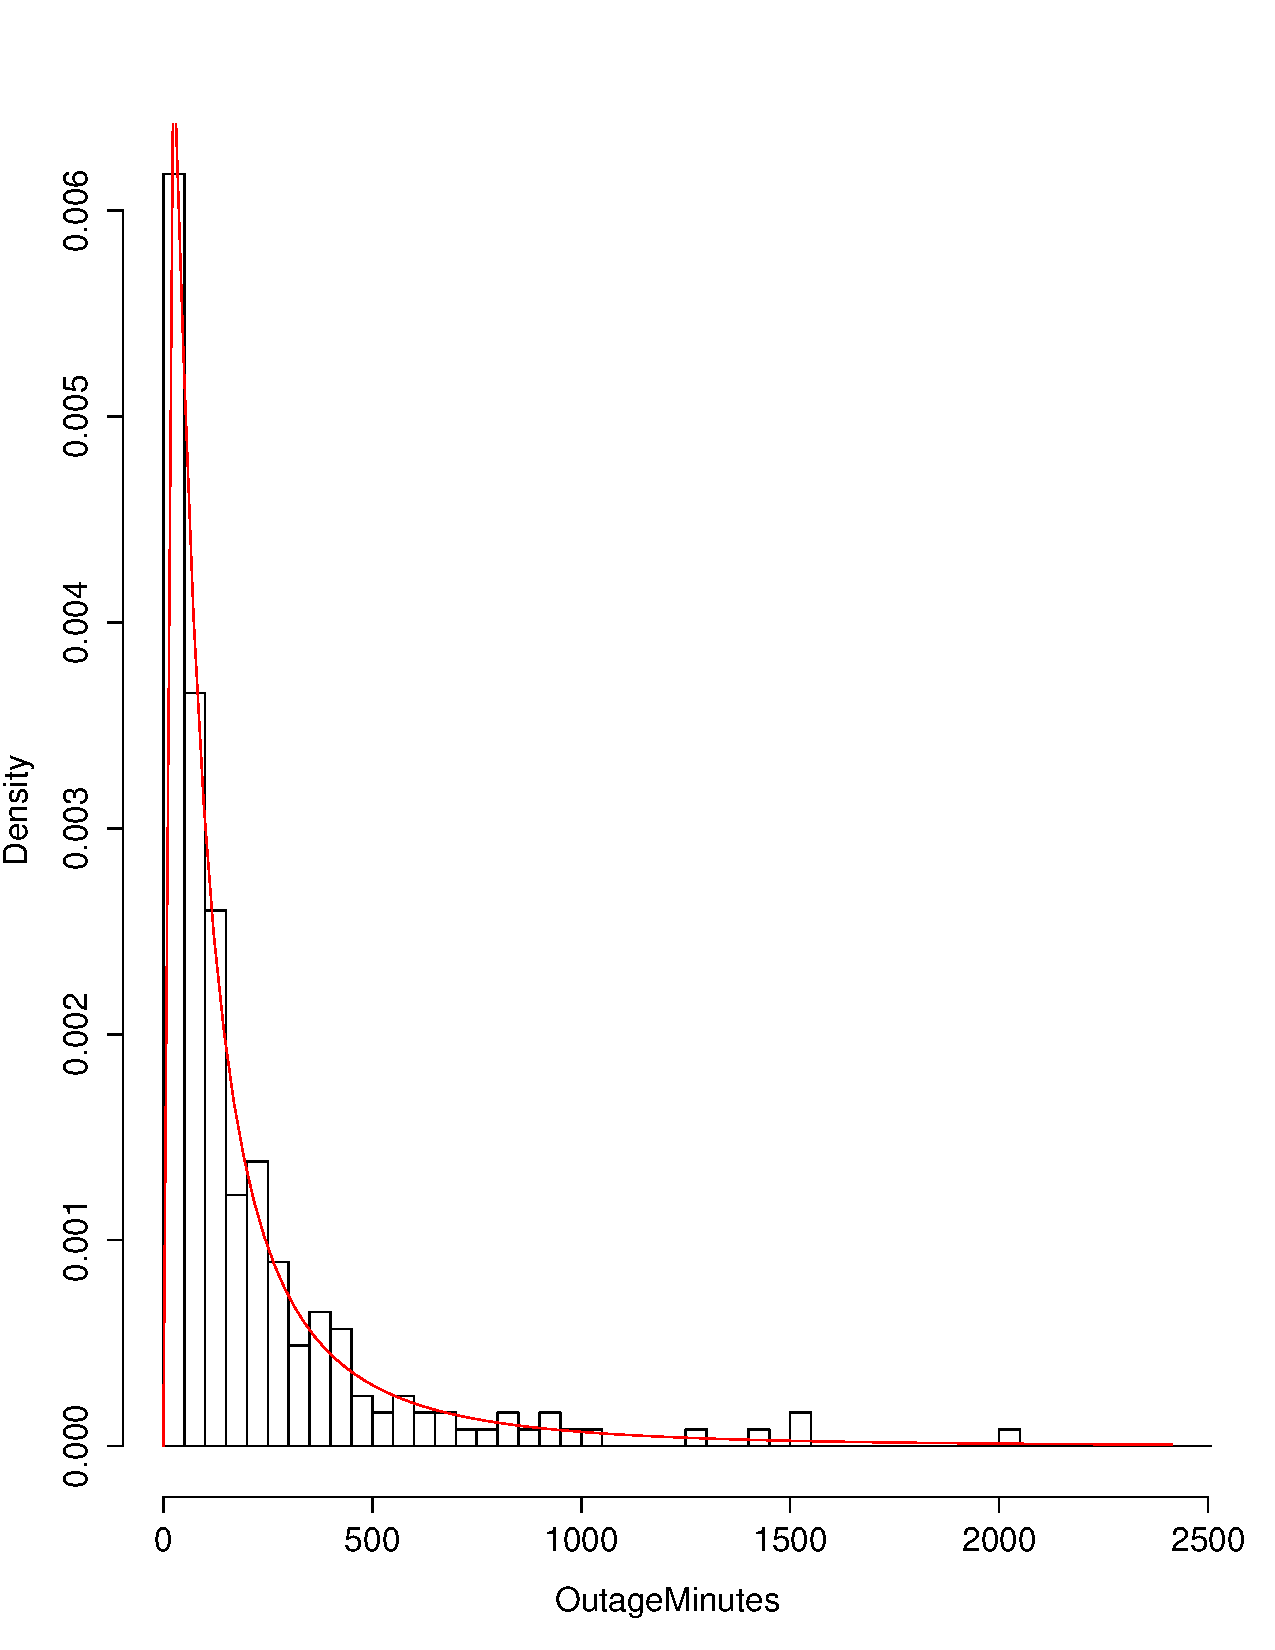
\includegraphics[height=9cm, width=9cm]{graphs/service/graph1.pdf} 
\end{center}
\end{figure}

\begin {table}
\begin{center}
\caption {Measures of location for outage service times \& distribution GoF details}
\label{tab:chap4tab5}
\begin{tabular}{| C{4cm} | C{4cm} |} \hline 
\textbf{Statistic} & \textbf{Value} 
\\ \hline Samples & 246
\\ \hline Mean & 314
\\ \hline Std Dev & 1414
\\ \hline Median & 105
\\ \hline Skew & 13.80
\\ \hline Distribution & log-normal
\\ \hline AD GoF p-value & 0.95
\\ \hline
\end{tabular}
\end{center}
\end{table}


Fig. \ref{fig:chap4fig2} shows a probability density function histogram for all 246 outage events with a fitted log-normal curve. 
Table \ref{tab:chap4tab5} lists the measure of location (i.e. mean, standard deviation, median and skew) for all outage events along with the distribution type and an Anderson-Darling goodness of fit p-value.

\subsection{Results - outage component}

\begin {table}
\begin{center}
\caption {Summary statistics for outage service times by component with log-normal GoF} 
\label{tab:chap4tab6}
\begin{tabular}{| C{2.5cm} | C{2.4cm} | C{2.9cm} | C{2cm} | C{2cm} |} \hline 
\textbf{Statistic} & \textbf{BSS/Social} & \textbf{Collaboration} & \textbf{Email} & \textbf{Mixed}
\\ \hline Samples & 16 & 34 & 152 & 43
\\ \hline \% Samples & 7 & 14 & 62 & 17
\\ \hline  Mean & 274 & 189 & 258 & 626
\\ \hline  Std Dev & 639 & 379 & 423 & 3261
\\ \hline  Median & 45 & 61.5 & 126.5 & 85
\\ \hline  Skew & 3.56 & 3.83 & 5.45 & 6.30
\\ \hline AD GoF (p) & 0.69 & 0.62 & 0.99 & 0.64
\\ \hline 
\end{tabular}
\end{center}
\end{table}

Table \ref{tab:chap4tab6} lists the summary statistics of outage events broken down by component. E-Mail recorded the highest proportion of all outages. BSS/social recorded had the lowest. Outages are most likely to happen in the E-mail component. \par

Due to the small number of samples (16) recorded for the BSS/social category, the goodness of fit value should be treated with caution. \par

\subsection{Results - outage type}

\begin {table}
\begin{center}
\caption {Summary statistics for outage service times by type with log-normal GoF} 
\label{tab:chap4tab7}
\begin{tabular}{| C{2.02cm} | C{1.9cm} | C{1.9cm} | C{1.9cm} | C{1.78cm} | C{1.9cm} |} \hline 
\textbf{Statistic} & \textbf{Configuration} & \textbf{Contention} & \textbf{Disaster} & \textbf{Network} & \textbf{Hardware}
\\ & \textbf{Manual} & \textbf{Concurrency} & \textbf{Recovery} & & \textbf{Other}
\\ \hline \# Samples & 74 & 64 & 36 & 49 & 23
\\ \hline  \% Samples & 30 & 26 & 15 & 20 & 9
\\ \hline Mean & 488 & 239 & 134 & 	315	& 243
\\ \hline Std Dev & 2488	& 469 & 161	& 591 	& 358
\\ \hline Median & 114.5	& 86	& 72	& 145	& 91
\\ \hline  Skew & 8.28	& 3.69	& 2.33	& 5.30	& 2.11
\\ \hline AD GoF (p) & 0.91 & 0.97 & 0.94 & 0.75 & 0.96
\\ \hline 
\end{tabular}
\end{center}
\end{table}

Table \ref{tab:chap4tab7} lists the summary statistics of outage events broken down by type. Configuration/Manual and Contention/Concurrency recorded the highest proportion of outages while Hardware/Other had the lowest. Outages are most likely to be either Configuration/Manual or Contention/Concurrency. 

Due to the small number of samples (23) for the Hardware/Other category, the goodness of fit value should be treated with caution. \par

\subsection{Results - Data centre location}

\begin {table}
\begin{center}
\caption {Summary statistics for outage service times by data centre with log-normal GoF} 
\label{tab:chap4tab8}
\begin{tabular}{| C{3cm} | C{3cm} | C{3cm} | C{3cm} |} \hline 
\textbf{Statistic} & \textbf{Data centre A} & \textbf{Data centre B}  & \textbf{Data centre C} 
\\ \hline Samples & 160 & 24 & 54 
\\ \hline \% Samples & 65 & 10 & 22
\\ \hline Mean & 224	& 188 	& 645
\\ \hline Std Dev & 313	& 280 & 2961
\\ \hline Median & 113.5	& 89.5	& 79.5
\\ \hline Skew & 2.93	& 2.89	& 6.67 
\\ \hline AD GoF (p) & 0.99 & 0.99 & 0.31 
\\ \hline 
\end{tabular}
\end{center}
\end{table}

Table \ref{tab:chap4tab8} lists the summary statistics of outage events broken down by data centre. Data Centre A recorded the highest proportion of outages, while Data centre B had the lowest. The remaining 3\% were from outages found in all thee data centres.  Outages are most likely to happen within Data Centre A.

Eight outages were found in all three data centres. Due to the small number of samples detailed analysis was not performed. Furthermore the researches felt it in was inappropriate to merge these eight samples into one of the existing data centre pools as this may confound analysis and results from a single data centre category. \par

\subsection{Discussion - outage service time distribution}

To answer the question how are the times of Cloud outage events distributed, an Anderson Darling goodness of fit test was conducted against a number of distributions; Exponential, Gamma, log-normal and Weibull. With the exception of log-normal,  the p values were very low, which indicated that these distribution types were a poor fit. For log-normal a p value was found to be 0.95. \par

In this case the hypothesis that the outage times are log-normal distributed is a surprisingly good fit. Fig. \ref{fig:chap4fig2} and Table \ref{tab:chap4tab5} clearly show that the distribution type is log-normal. This finding further expands the applicability of the use of the log-normal distribution of model repair times. It is known that repairable systems typically refer to mechanical, electric and electronic systems. However given the above results we can now include software systems as another subtype.\par

It is also worth noting that the mean outage time is approximately 314 minutes, which indicates that resolution of an outage in complex system architecture is a non-trivial task. Additionally with a standard deviation found to be approximately 1414 minutes and a skew value of 13.80, clearly indicates that there is a high level of dispersion within the dataset. \par

Given the nature of Cloud computing, new code updates and configuration changes are made on a regular basis. It is not uncommon for an enterprise to introduce changes on a bi-weekly or monthly basis. Therefore with this high level of system activity it is not unsurprising that outages can occur frequently. If a state of the art outage tracking system were introduced, it would be interesting to determine overall as both process improvements were made coupled with underlying code stability to observe the overall affect on both the distribution type and shape. This would provide a concrete answer to questions such as: what impact do specific process improvements make to overall outage times? As a business where do resources need to be deployed to improve platform stability: Development, Operations or Quality Assurance? \par

\subsection{Discussion - outage component}

Examining outages by component can give insight as to which component are likely to exhibit outages and whether these times vary by component. \par

Table \ref{tab:chap4tab6} provides summary details of outages by component. It was noted that mixed components had the highest mean outage time with 627 minutes, followed by BSS/social, Mail with 274 \& 258 respectively and Collaboration with 189 minutes. Consequently mixed components also has the highest standard deviation and skew. In all cases, each component class had a good fit to a log-normal distribution, with the email category fitting best with a p value of 0.99. However the BBS-Social category has a low number of samples, therefore the goodness of fit assessment should be treated with some caution. \par

Based on these results it is clear that the email component has the highest proportion of outages. Tiger teams should review the root cause of each outage related to the email component.  This will gain understanding as to the what types of failures contribute most to email outage events. Triangulating each outage event against the failure type and data centre location can help business and operations teams resource their crisis teams on a per component basis.

Secondly the results show that mixed components have the highest mean outage time. This result seems logical, given that when an outage occurs across common infrastructure and/or multiple components that the repair time is greater. There are many systems to check and repair as part of the remediation process. To verify, the individual reports were checked for mixed component failures. It was found that one outage took multiple days to resolve. Hence skewing the overall mean time. While this data point may be considered an outlier in the classic sense, given this was a real fault, it must be included as part of analysis. Tiger teams should determine the the root cause of each outage to intersect failure type and data centre to understand common failure patterns. \par


\subsection{Discussion - outage type}
Examining outages by type gives a deeper understanding of what types of problems are likely to cause an outage within a Cloud infrastructure. Table \ref{tab:chap4tab7} provides this insight. \par

Significantly Configuration/Manual had the highest expected outage time with 489 minutes, with Network next highest with 315 minutes. Contention/Concurrency, Hardware and Disaster recovery had expected outages times of 239, 243 and 134 minutes respectively. Finally the outage times of each category were fitted with a log-normal distribution. In each case the hypothesis of whether a log-normal distribution was a suitable distribution could not be rejected. However one caveat is that the Hardware/Other category had a low number of samples, so this result must be treated with caution. \par

It is clear that issues related to Configuration/Manual contribute most to the overall number of outages but also take the longest to resolve.  Given the relative complexity of the overall Cloud architecture it is apparent that a system of managed configuration changes is required. Firstly to ensure that for all configuration changes made, that there is a commit and rollback feature to ensure that that harmful (extreme) configuration settings can be reversed if required. Additionally tiger teams should implement a system, which can monitor real-time configuration changes across all data centres.  \par

With any distributed system the network health plays an important role in system stability. The network issues studied fell into two main categories: network congestion and temporary network outages. For congestion issues, business and operations teams need to define clear bandwidth capacity requirements to ensure that their infrastructure has the bandwidth to meet the demands of their existing user base and future subscription signings. The underlying application code and middleware stack should have additional resiliency added to ensure that temporary outages do not cause cascade failures.  \par

\subsection{Discussion - data centre location}

Table \ref{tab:chap4tab8} provides summary details of outages by data centre. As discussed previously in our case study outline, user concurrency varies by data centre. Data Centre C had the highest mean outage time with 645 minutes, while data centre's A \& B had mean outages times of 224 and 188 respectively. All three data centre outage times were modelled with a log-normal distribution and both data centre A \& B were an excellent fit. Each had a  p value of 0.99. Data centre C faired worst in terms of fit with a p value of 0.31. Even with this value the hypothesis of whether a log normal distribution is a suitable fit cannot be rejected. \par

In some ways the above results are expected, it seems intuitive that a high use data centre would incur the most outages due to the high level of customer activity, however even with all these outages the mean outage time is 224 minutes, which is approximately 90 minutes less than the overall mean. What appears somewhat counter intuitive is that data centre C has the second highest number of outages and the highest mean outage time. From closer inspection the mean outage time of data centre C is due to a small number of outages with high durations. Finally it is worth noting that Data centre B has the lowest number of outage events and the lowest mean outage time.\par

In the context of software delivery to multiple data centres, the same code is released to each system. Clearly customers are impacted in different ways depending on which data centre is used. With this knowledge, tiger teams can investigate in two areas. Firstly does the underlying customer use case of each data centre vary? Secondly a root and branch investigation of each data centre configuration should be conducted and compared for discrepancies, with specific focus on the configuration of the email component. \par


% % % % % % % % % % % % % % % % % % % % % % % % % % % % % % % % % % % % % % % % % % % % % % % % % % % % % %
%------------------------------------------- CONCLUSIONS --------------------------------------------------
% % % % % % % % % % % % % % % % % % % % % % % % % % % % % % % % % % % % % % % % % % % % % % % % % % % % % %

\section{Conclusion}
The purpose of our case studies conducted in this chapter was to model the inter-arrival time and service time duration of a data set of Cloud outage events. Our key aim was to understand if either or both durations could be modelled by a known probability distribution. It was found that the Pareto distribution is a useful distribution for modelling the inter-arrival times of Cloud outages. It was also found that the log-normal distribution is a useful distribution for modelling repair times of SaaS outages. The findings of this study support previous research particularly in the field of system reliability and repair times. \par

Previous studies have shown that shown that Cloud outages are an infrequent occurrence. Additionally we show that the log-normal distribution is a useful tool for modelling repair times in mechanical and electronic maintainable systems. \par

This work adds to the existing literature in the area of modelling inter-arrival and service times. Our contributions provide additional results as to how repair times can vary between failure type, component and the data centre used at the time of a Cloud outage. \par

In future SMEs can assess their outage data to understand the core issues that effect their underlying service platform. A specific operations framework can then be developed to allow micro teams and SMEs to focus on specific areas of their architecture or business process, which impede reliability. Likewise, by usage of this framework on an iterative basis, an SME can then set realistic remediation targets. \par

In our next chapter we shall assess the results of our inter-arrival and service models to understand how Cloud failures can be simulated over a period of time. Additionally we consider how DevOps can be deployed using this simulation model. \par


% ---------------------------------------------------------------------------
% ----------------------- end of thesis sub-document ------------------------
% ---------------------------------------------------------------------------
